% !TeX root = RJwrapper.tex
\title{Predicting Motor Vehicle Collisions in New York City}
\author{by Alex Fung, Viswesh Krishnamurthy, Tony Lee, Patrick Osborne}

\maketitle


\begin{Schunk}
\begin{Soutput}
#> [1] 56000
\end{Soutput}
\end{Schunk}

\begin{Schunk}
\begin{Sinput}
#code below IS shown in final document
\end{Sinput}
\end{Schunk}

\hypertarget{abstract}{%
\subsection{Abstract}\label{abstract}}

Technological progress in the world has unarguably improved the quality
of life for the average person in many ways. The age of the automobile
has shaped the way in which work, play and live our lives. Roadways,
buildings, cities and entire countries have been designed to accommodate
motor vehicles. As automobile technology has advanced making cars faster
and capable of more advanced maneuvers, so has our concern with the
safety of these vehicles. Entire disciplines such as traffic management
are devoted to optimizing numerous factors to ensure the safe and
efficient movement of people and goods. As we move into the age of data,
all stakeholders in the automobile industry must effectively collect and
utilize the wealth of information available to better meet their goals
if progress is to continue. In this project, we take the position of a
law enforcement agency, the New York City Police Department, as they
seek to best utilize their resources in the context of responding to
traffic collisions in the city.

\hypertarget{background}{%
\subsection{Background}\label{background}}

At the end of 2017 in New York City, there were 1,923,041 cars
registered to residents of the city.
(\url{https://nyc.streetsblog.org/2018/10/03/car-ownership-continues-to-rise-under-mayor-de-blasio/})
This already-significant number does not include the heavy flow of
vehicles of those who visit the city or are simply passing through. By
contrast, the New York City Police Department (NYPD) budgets for a
headcount of 35,822 uniformed officers
(\url{http://council.nyc.gov/budget/wp-content/uploads/sites/54/2017/03/056-NYPD.pdf}
- page 4), distributed across 77 police precincts (geographic divisions
of the city). On-duty officers/traffic enforcement agents are allocated
to each precinct to enforce traffic laws and handle emergency and
administrative response to traffic incidents (such as collisions). NYC
has been collecting traffic data, including specific data on vehicle
collisions since 2014 to support ``Vision Zero'' , a traffic safety
initiative which has the goal of eliminating traffic fatalities.
(\url{https://data.cityofnewyork.us/Public-Safety/Motor-Vehicle-Collisions-Crashes/h9gi-nx95/data})

\hypertarget{objective}{%
\subsection{Objective}\label{objective}}

The objective of our analysis is to develop a supervised, prediction
model using Machine Learning techniques and the CRISP-DM framework (cite
textbook) on the available collision data to predict whether there will
be a collision in a specified police precinct at a specified time. The
intent of predicting this data is to inform the NYPD's optimal
assignment of limited officers and resources across the 77 police
precincts.

\hypertarget{data-analysis}{%
\subsection{Data Analysis}\label{data-analysis}}

The data set that supports this analysis is sourced from the NYC Open
Data project. The title of the data set is ``Motor Vehicle Collisions --
Crashes''. It contains entries for every collision recorded within New
York City limits by NYPD agents beginning July 1st, 2012 up to the
present day. There are approximately 1.65 million entries in the data
set.

\hypertarget{data-dictionary}{%
\subsection{Data Dictionary}\label{data-dictionary}}

Data dictionary sourced from
\url{https://data.cityofnewyork.us/Public-Safety/Motor-Vehicle-Collisions-Crashes/h9gi-nx95/data}
- ``MVCollisionsDataDictionary\_20190813\_ERD.xlsx''.

\begin{table}

\caption{\label{tab:data-dictionary}Data Dictionary - Motor Vehicle Collisions – Crashes}
\centering
\begin{tabular}[t]{l|l}
\hline
Feature & Feature.Description\\
\hline
COLLISION\_ID & Unique record code generated by system\\
\hline
ACCIDENT\_DATE & Occurrence date of collision\\
\hline
ACCIDENT\_TIME & Occurrence time of collision\\
\hline
BOROUGH & Borough where collision occurred\\
\hline
ZIP CODE & Postal code of incident occurrence\\
\hline
LATITUDE & Latitude coordinate for Global Coordinate System, WGS 1984\\
\hline
LONGITUDE & Longitude coordinate for Global Coordinate System, WGS 1984\\
\hline
LOCATION & Latitude , Longitude pair\\
\hline
ON STREET NAME & Street on which the collision occurred\\
\hline
CROSS STREET NAME & Nearest cross street to the collision\\
\hline
OFF STREET NAME & Street address if known\\
\hline
NUMBER OF PERSONS INJURED & Number of persons injured\\
\hline
NUMBER OF PERSONS KILLED & Number of persons killed\\
\hline
NUMBER OF PEDESTRIANS INJURED & Number of pedestrians injured\\
\hline
NUMBER OF PEDESTRIANS KILLED & Number of pedestrians killed\\
\hline
NUMBER OF CYCLIST INJURED & Number of cyclists injured\\
\hline
NUMBER OF CYCLIST KILLED & Number of cyclists killed\\
\hline
NUMBER OF MOTORIST INJURED & Number of vehicle occupants injured\\
\hline
NUMBER OF MOTORIST KILLED & Number of vehicle occupants killed\\
\hline
CONTRIBUTING FACTOR VEHICLE 1 & Factors contributing to the collision for designated vehicle\\
\hline
CONTRIBUTING FACTOR VEHICLE 2 & Factors contributing to the collision for designated vehicle\\
\hline
CONTRIBUTING FACTOR VEHICLE 3 & Factors contributing to the collision for designated vehicle\\
\hline
CONTRIBUTING FACTOR VEHICLE 4 & Factors contributing to the collision for designated vehicle\\
\hline
CONTRIBUTING FACTOR VEHICLE 5 & Factors contributing to the collision for designated vehicle\\
\hline
VEHICLE TYPE CODE 1 & Type of vehicle based on the selected vehicle category\\
\hline
VEHICLE TYPE CODE 2 & Type of vehicle based on the selected vehicle category\\
\hline
VEHICLE TYPE CODE 3 & Type of vehicle based on the selected vehicle category\\
\hline
VEHICLE TYPE CODE 4 & Type of vehicle based on the selected vehicle category\\
\hline
VEHICLE TYPE CODE 5 & Type of vehicle based on the selected vehicle category\\
\hline
\end{tabular}
\end{table}

\newpage

\hypertarget{initial-data-exploration-and-cleaning}{%
\subsection{Initial Data Exploration and
Cleaning}\label{initial-data-exploration-and-cleaning}}

{[}SUMMARY OF DATA INSERT TEXT{]}

\scalebox{0.6}{
\begin{tabular}{llllll}
  \hline
     CRASH.DATE &   CRASH.TIME &          BOROUGH &    ZIP.CODE &    LATITUDE &   LONGITUDE \\ 
  \hline
01/21/2014:   1161   & 16:00  :  24074   &              :499865   & Min.   :10000   & Min.   : 0.00   & Min.   :-201.36   \\ 
  11/15/2018:   1065   & 17:00  :  23613   & BRONX        :160097   & 1st Qu.:10304   & 1st Qu.:40.67   & 1st Qu.: -73.98   \\ 
  12/15/2017:    999   & 15:00  :  23171   & BROOKLYN     :355543   & Median :11206   & Median :40.72   & Median : -73.93   \\ 
  05/19/2017:    974   & 18:00  :  21767   & MANHATTAN    :273153   & Mean   :10828   & Mean   :40.69   & Mean   : -73.87   \\ 
  01/18/2015:    961   & 14:00  :  21258   & QUEENS       :305510   & 3rd Qu.:11237   & 3rd Qu.:40.77   & 3rd Qu.: -73.87   \\ 
  02/03/2014:    960   & 13:00  :  19732   & STATEN ISLAND: 49124   & Max.   :11697   & Max.   :43.34   & Max.   :   0.00   \\ 
  (Other)   :1637172   & (Other):1509677   &  & NA's   :500110   & NA's   :199425   & NA's   :199425   \\ 
   \hline
\end{tabular}
}

{[}1{]} " \n" \scalebox{0.6}{
\begin{tabular}{llll}
  \hline
                          LOCATION &                          ON.STREET.NAME &                        CROSS.STREET.NAME &                                 OFF.STREET.NAME \\ 
  \hline
                              : 199425   &                                 : 323553   &                                 : 555996   &                                         :1411905   \\ 
  POINT (0 0)                   :   1113   & BROADWAY                        :  16258   & 3 AVENUE                        :   9846   & 772       EDGEWATER ROAD                :    375   \\ 
  POINT (-74.038086 40.608757)  :    670   & ATLANTIC AVENUE                 :  14401   & BROADWAY                        :   9685   & 110-00    ROCKAWAY BOULEVARD            :    244   \\ 
  POINT (-73.9845292 40.6960346):    586   & 3 AVENUE                        :  11761   & 2 AVENUE                        :   8425   & 2800      VICTORY BOULEVARD             :    221   \\ 
  POINT (-73.98453 40.696033)   :    574   & NORTHERN BOULEVARD              :  11460   & 5 AVENUE                        :   7052   &                                         :    183   \\ 
  POINT (-73.91282 40.861862)   :    545   & BELT PARKWAY                    :  11302   & 7 AVENUE                        :   6634   & 2100      BARTOW AVENUE                 :    158   \\ 
  (Other)                       :1440379   & (Other)                         :1254557   & (Other)                         :1045654   & (Other)                                 : 230206   \\ 
   \hline
\end{tabular}
} {[}1{]} " \n" \scalebox{0.6}{
\begin{tabular}{llll}
  \hline
NUMBER.OF.PERSONS.INJURED & NUMBER.OF.PERSONS.KILLED & NUMBER.OF.PEDESTRIANS.INJURED & NUMBER.OF.PEDESTRIANS.KILLED \\ 
  \hline
Min.   : 0.0000   & Min.   :0.000000   & Min.   : 0.00000   & Min.   :0.000000   \\ 
  1st Qu.: 0.0000   & 1st Qu.:0.000000   & 1st Qu.: 0.00000   & 1st Qu.:0.000000   \\ 
  Median : 0.0000   & Median :0.000000   & Median : 0.00000   & Median :0.000000   \\ 
  Mean   : 0.2634   & Mean   :0.001174   & Mean   : 0.05092   & Mean   :0.000641   \\ 
  3rd Qu.: 0.0000   & 3rd Qu.:0.000000   & 3rd Qu.: 0.00000   & 3rd Qu.:0.000000   \\ 
  Max.   :43.0000   & Max.   :8.000000   & Max.   :27.00000   & Max.   :6.000000   \\ 
  NA's   :17   & NA's   :31   &  &  \\ 
   \hline
\end{tabular}
} {[}1{]} " \n" \scalebox{0.6}{
\begin{tabular}{llll}
  \hline
NUMBER.OF.CYCLIST.INJURED & NUMBER.OF.CYCLIST.KILLED & NUMBER.OF.MOTORIST.INJURED & NUMBER.OF.MOTORIST.KILLED \\ 
  \hline
Min.   :0.00000   & Min.   :0.00e+00   & Min.   : 0.000   & Min.   :0.000000   \\ 
  1st Qu.:0.00000   & 1st Qu.:0.00e+00   & 1st Qu.: 0.000   & 1st Qu.:0.000000   \\ 
  Median :0.00000   & Median :0.00e+00   & Median : 0.000   & Median :0.000000   \\ 
  Mean   :0.02062   & Mean   :8.34e-05   & Mean   : 0.192   & Mean   :0.000452   \\ 
  3rd Qu.:0.00000   & 3rd Qu.:0.00e+00   & 3rd Qu.: 0.000   & 3rd Qu.:0.000000   \\ 
  Max.   :4.00000   & Max.   :2.00e+00   & Max.   :43.000   & Max.   :5.000000   \\ 
   \hline
\end{tabular}
} {[}1{]} " \n" \scalebox{0.6}{
\begin{tabular}{llll}
  \hline
               CONTRIBUTING.FACTOR.VEHICLE.1 &                CONTRIBUTING.FACTOR.VEHICLE.2 &                CONTRIBUTING.FACTOR.VEHICLE.3 &                CONTRIBUTING.FACTOR.VEHICLE.4 \\ 
  \hline
Unspecified                   :599544   & Unspecified                   :1193786   &                               :1536917   &                               :1621113   \\ 
  Driver Inattention/Distraction:308381   &                               : 222550   & Unspecified                   :  98931   & Unspecified                   :  20912   \\ 
  Failure to Yield Right-of-Way : 94090   & Driver Inattention/Distraction:  75420   & Other Vehicular               :   1949   & Other Vehicular               :    364   \\ 
  Following Too Closely         : 82937   & Other Vehicular               :  27258   & Driver Inattention/Distraction:   1424   & Following Too Closely         :    237   \\ 
  Backing Unsafely              : 62951   & Failure to Yield Right-of-Way :  14284   & Following Too Closely         :   1298   & Driver Inattention/Distraction:    175   \\ 
  Other Vehicular               : 52108   & Following Too Closely         :  14009   & Fatigued/Drowsy               :    853   & Fatigued/Drowsy               :    170   \\ 
  (Other)                       :443281   & (Other)                       :  95985   & (Other)                       :   1920   & (Other)                       :    321   \\ 
   \hline
\end{tabular}
} {[}1{]} " \n" \scalebox{0.6}{
\begin{tabular}{llll}
  \hline
               CONTRIBUTING.FACTOR.VEHICLE.5 &  COLLISION\_ID &                          VEHICLE.TYPE.CODE.1 &                          VEHICLE.TYPE.CODE.2 \\ 
  \hline
                              :1637609   & Min.   :     22   & PASSENGER VEHICLE                  :715236   & PASSENGER VEHICLE                  :537550   \\ 
  Unspecified                   :   5361   & 1st Qu.:1038275   & SPORT UTILITY / STATION WAGON      :313500   &                                    :273620   \\ 
  Other Vehicular               :     96   & Median :3457776   & Sedan                              :172288   & SPORT UTILITY / STATION WAGON      :237846   \\ 
  Following Too Closely         :     51   & Mean   :2808228   & Station Wagon/Sport Utility Vehicle:140852   & Sedan                              :128269   \\ 
  Fatigued/Drowsy               :     41   & 3rd Qu.:3868829   & TAXI                               : 50670   & Station Wagon/Sport Utility Vehicle:108877   \\ 
  Driver Inattention/Distraction:     40   & Max.   :4280357   & VAN                                : 26540   & (Other)                            :357127   \\ 
  (Other)                       :     94   &  & (Other)                            :224206   & NA's                               :     3   \\ 
   \hline
\end{tabular}
} {[}1{]} " \n" \scalebox{0.6}{
\begin{tabular}{llll}
  \hline
                         VEHICLE.TYPE.CODE.2 &                          VEHICLE.TYPE.CODE.3 &                          VEHICLE.TYPE.CODE.4 &                          VEHICLE.TYPE.CODE.5 \\ 
  \hline
PASSENGER VEHICLE                  :537550   &                                    :1507965   &                                    :1593350   &                                    :1632527   \\ 
                                     :273620   & PASSENGER VEHICLE                  :  63655   & PASSENGER VEHICLE                  :  24743   & PASSENGER VEHICLE                  :   5476   \\ 
  SPORT UTILITY / STATION WAGON      :237846   & SPORT UTILITY / STATION WAGON      :  33161   & SPORT UTILITY / STATION WAGON      :  14375   & SPORT UTILITY / STATION WAGON      :   3138   \\ 
  Sedan                              :128269   & Sedan                              :  11698   & Sedan                              :   2598   & Sedan                              :    668   \\ 
  Station Wagon/Sport Utility Vehicle:108877   & Station Wagon/Sport Utility Vehicle:   9730   & Station Wagon/Sport Utility Vehicle:   2102   & Station Wagon/Sport Utility Vehicle:    548   \\ 
  (Other)                            :357127   & UNKNOWN                            :   3285   & TAXI                               :   1681   & TAXI                               :    246   \\ 
  NA's                               :     3   & (Other)                            :  13798   & (Other)                            :   4443   & (Other)                            :    689   \\ 
   \hline
\end{tabular}
}

Based on what we know about the data set from the specifications at NYC
Open Data and the data dictionary, we have decided to perform some
initial cleaning steps.

Our analytics problem is to predict whether there will be a collision at
a specific time (time including a time of the day, day of the year and
calendar year). In this context, we will first look at the
``CRASH.DATE'' graph. Thinking about the scheduling of police resource,
we assume that this happens in advance, on a hour-by-hour and day-by-day
basis. We assume that resources are not scheduled on a year-by-year
basis due to uncertainty in staffing, budget, etc. We therefore examine
the data to see whether we should include the year at all. Including the
year would treat the data set as a time-series, years ranging from
2012-2020. Alternatively, we could drop the year and group all
occurrences on the same day in the same bin, possibly enhancing our
prediction.

To decide, we plot the dates and look for trends. If trends repeat
annually, we will drop the year as this trend will be preserved when we
combine. If the trend does not repeat annually (extends over the whole
range of dates) then we will not combine year as we will lose this
information when dropping year.

\begin{Schunk}
\begin{figure}

{\centering 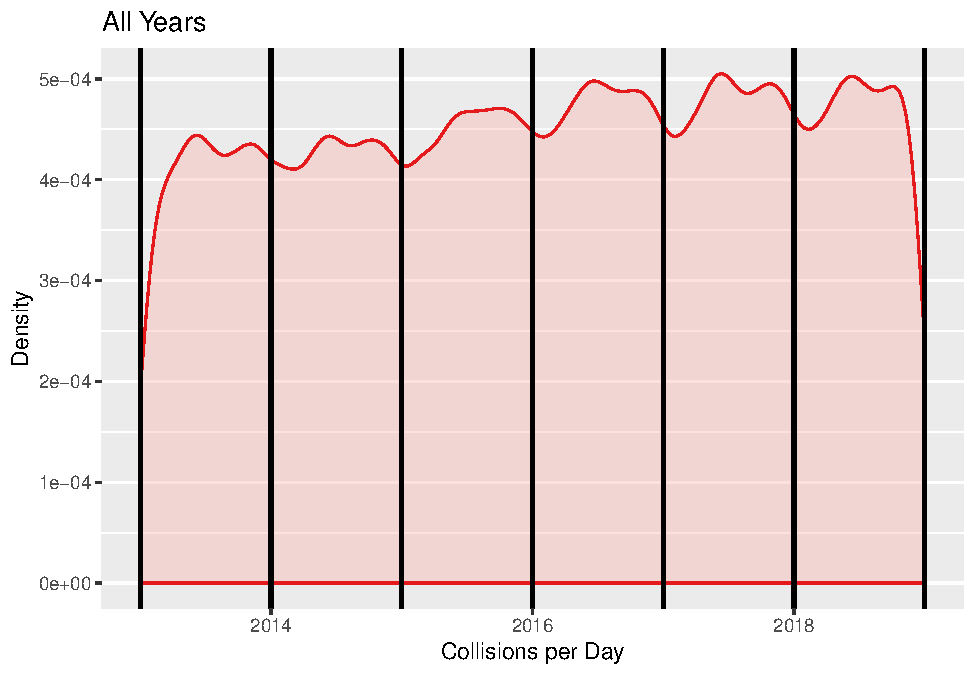
\includegraphics{RMarkdown-Group_10-Assignment_1_files/figure-latex/unnamed-chunk-4-1} 

}

\caption[Collisions per Day - All Years]{Collisions per Day - All Years}\label{fig:unnamed-chunk-4}
\end{figure}
\end{Schunk}

The vertical black lines in the ``All Years'' plot represent the start
of each year. As you can see from the plot, there is a noticeable
repeating trend in each year (between the black lines) with a decrease
in collisions at the start of each year, followed by various other
increase/decreases. As we are more interested in capturing this
repeating annual trend than year-over-year changes, we will combine all
data into a representation of one year. Additionally, we will drop years
2012 and 2020 (the first and last years in the data set) to avoid
over/under-representing specific months in the combined-year data set.
This leaves us with the ``Years Combined'' data set plotted below.

We use the following code to keep only data in 2013 onwards and in prior
to 2020, as mentioned.

\begin{Schunk}
\begin{Sinput}
raw_crash_dates_df <- raw_crash_dates_df[raw_crash_dates_df$raw_crash_dates > "2013-01-01", ]
raw_crash_dates_df <- raw_crash_dates_df[raw_crash_dates_df$raw_crash_dates < "2020-01-01", ]
\end{Sinput}
\end{Schunk}

\begin{Schunk}
\begin{figure}

{\centering 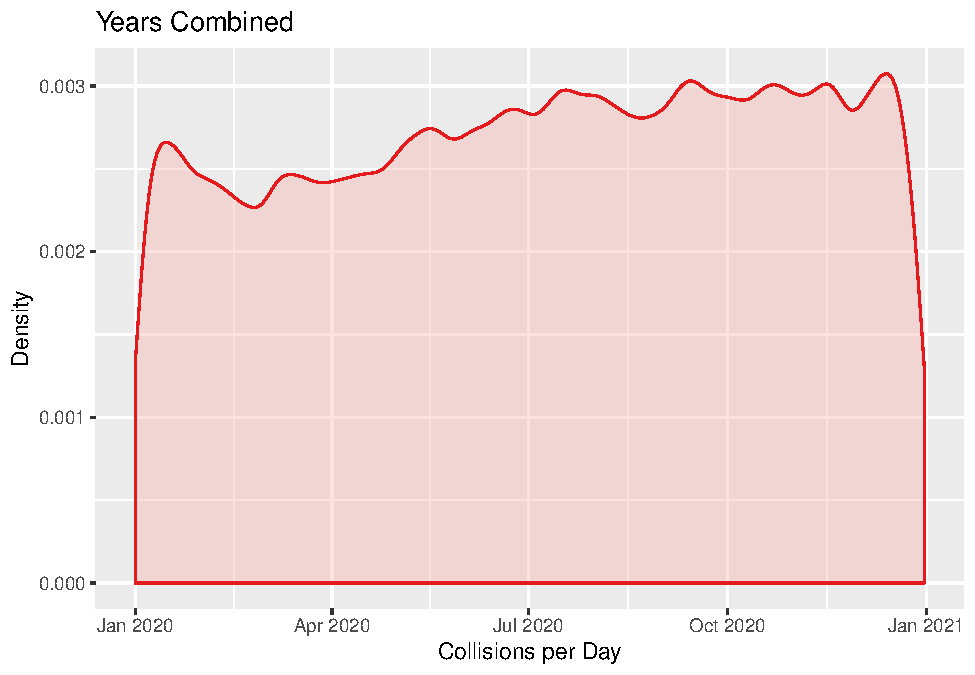
\includegraphics{RMarkdown-Group_10-Assignment_1_files/figure-latex/unnamed-chunk-6-1} 

}

\caption[Collisions per Day - Years Combined]{Collisions per Day - Years Combined}\label{fig:unnamed-chunk-6}
\end{figure}
\end{Schunk}

{[}INSERT WRITEUP ABOUT DATA CLEANING AND PREP HERE{]}

\hypertarget{cleaned-data-exploration}{%
\subsection{Cleaned Data Exploration}\label{cleaned-data-exploration}}

{[}TEXT ABOUT EXPLORING THE DATA{]}

\#density plot

\begin{Schunk}
\begin{figure}

{\centering \includegraphics{RMarkdown-Group_10-Assignment_1_files/figure-latex/data-exploration-1} 

}

\caption[Plots of Selected Features]{Plots of Selected Features}\label{fig:data-exploration}
\end{figure}
\end{Schunk}

\begin{Schunk}
\begin{Sinput}
#crash_dates <- as.Date(raw_crashes_data$CRASH.DATE, "%m/%d/%Y")
#ggplot(raw_crashes_data, aes(x=CRASH.DATE))
\end{Sinput}
\end{Schunk}

\hypertarget{document-style-attribution}{%
\subsection{Document Style
Attribution}\label{document-style-attribution}}

This document was generated using a modified version of the
``RJournal.sty'' file provided by the The R Foundation at
\url{https://journal.r-project.org/submissions.html}.

The document can be regenerated in RStudio by Knitting the provided ``R
Markdown-Group 10-Assignment 1.Rmd'' file with the provided
``RJournal.sty'' file in the same directory.

\hypertarget{default-r-markdown-code-below}{%
\section{DEFAULT R MARKDOWN CODE
BELOW}\label{default-r-markdown-code-below}}

\hypertarget{r-markdown}{%
\subsection{R Markdown}\label{r-markdown}}

This is an R Markdown document. Markdown is a simple formatting syntax
for authoring HTML, PDF, and MS Word documents. For more details on
using R Markdown see \url{http://rmarkdown.rstudio.com}.

When you click the \textbf{Knit} button a document will be generated
that includes both content as well as the output of any embedded R code
chunks within the document. You can embed an R code chunk like this:

\begin{Schunk}
\begin{Sinput}
summary(cars)
\end{Sinput}
\begin{Soutput}
#>      speed           dist       
#>  Min.   : 4.0   Min.   :  2.00  
#>  1st Qu.:12.0   1st Qu.: 26.00  
#>  Median :15.0   Median : 36.00  
#>  Mean   :15.4   Mean   : 42.98  
#>  3rd Qu.:19.0   3rd Qu.: 56.00  
#>  Max.   :25.0   Max.   :120.00
\end{Soutput}
\end{Schunk}

\hypertarget{including-plots}{%
\subsection{Including Plots}\label{including-plots}}

You can also embed plots, for example:

\begin{Schunk}

\includegraphics{RMarkdown-Group_10-Assignment_1_files/figure-latex/pressure-1} \end{Schunk}

Note that the \texttt{echo\ =\ FALSE} parameter was added to the code
chunk to prevent printing of the R code that generated the plot.


\address{%
Alex Fung\\
\\
\\
}


\address{%
Viswesh Krishnamurthy\\
\\
\\
}


\address{%
Tony Lee\\
\\
\\
}


\address{%
Patrick Osborne\\
\\
\\
}


